% !TEX root = template.tex

\section{Processing Pipeline}
The proposed approach aims at exploiting the temporal and spatial information in the Doppler traces obtained from the raw WiFi signals in order to perform an activity recognition and person identification task.

First the raw Doppler spectrum are collected from multiple antennas and processed to generate the input samples for our neural network. The CSI measurements associated with the different antennas are grouped together and each activity sequence is segmented into temporal windows of fixed length. Then the dataset is split into training, validation and test set, ensuring that the model is evaluated on different portions of the activity sequences while avoiding excessive overlapping between the samples. We then implemented two neural networks, one using a self-supervised approach for activity recognition and person identification, while the other using a supervised contrastive framework in order to be more robust on the activity recognition task.

In the first approach, data augmentation is applied to the signal windows through random transformations performed independently on each antenna. Samples originating from the same window, but captured by different antennas, are then treated as positive keys by the NT-Xent loss function, which is adapted to accommodate more than two positive keys. Consequently, in the initial phase, a neural network consisting of a backbone and a head undergoes self-supervised contrastive pretraining. The backbone learns to extract the signal features, deriving an optimal representation for each environment-person-activity association. Finally, this pre-trained backbone is coupled with two distinct heads: one for PI and one for AR.

The pipeline of this approach is illustrated in Figure~\ref{fig:FirstPipeline}

The second approach instead is divided in different stages: the first consist of a supervised contrastive pre-training phase. During this step, the network learns a compact representation of the Doppler traces by using the activity label to bring samples belonging to the same class closer in the embedding space. After this step, the feature extractor is transferred to a classification network, the parameters of the pre-training are frozen and only the final classification layer is optimized. By doing that the final model gives in output the predicted activity, while being very robust and reducing the risk of overfitting.

The complete pipeline of this second approach is illustrated in Figure~\ref{fig:SupCon}.
\begin{figure}[h]
    \centering
    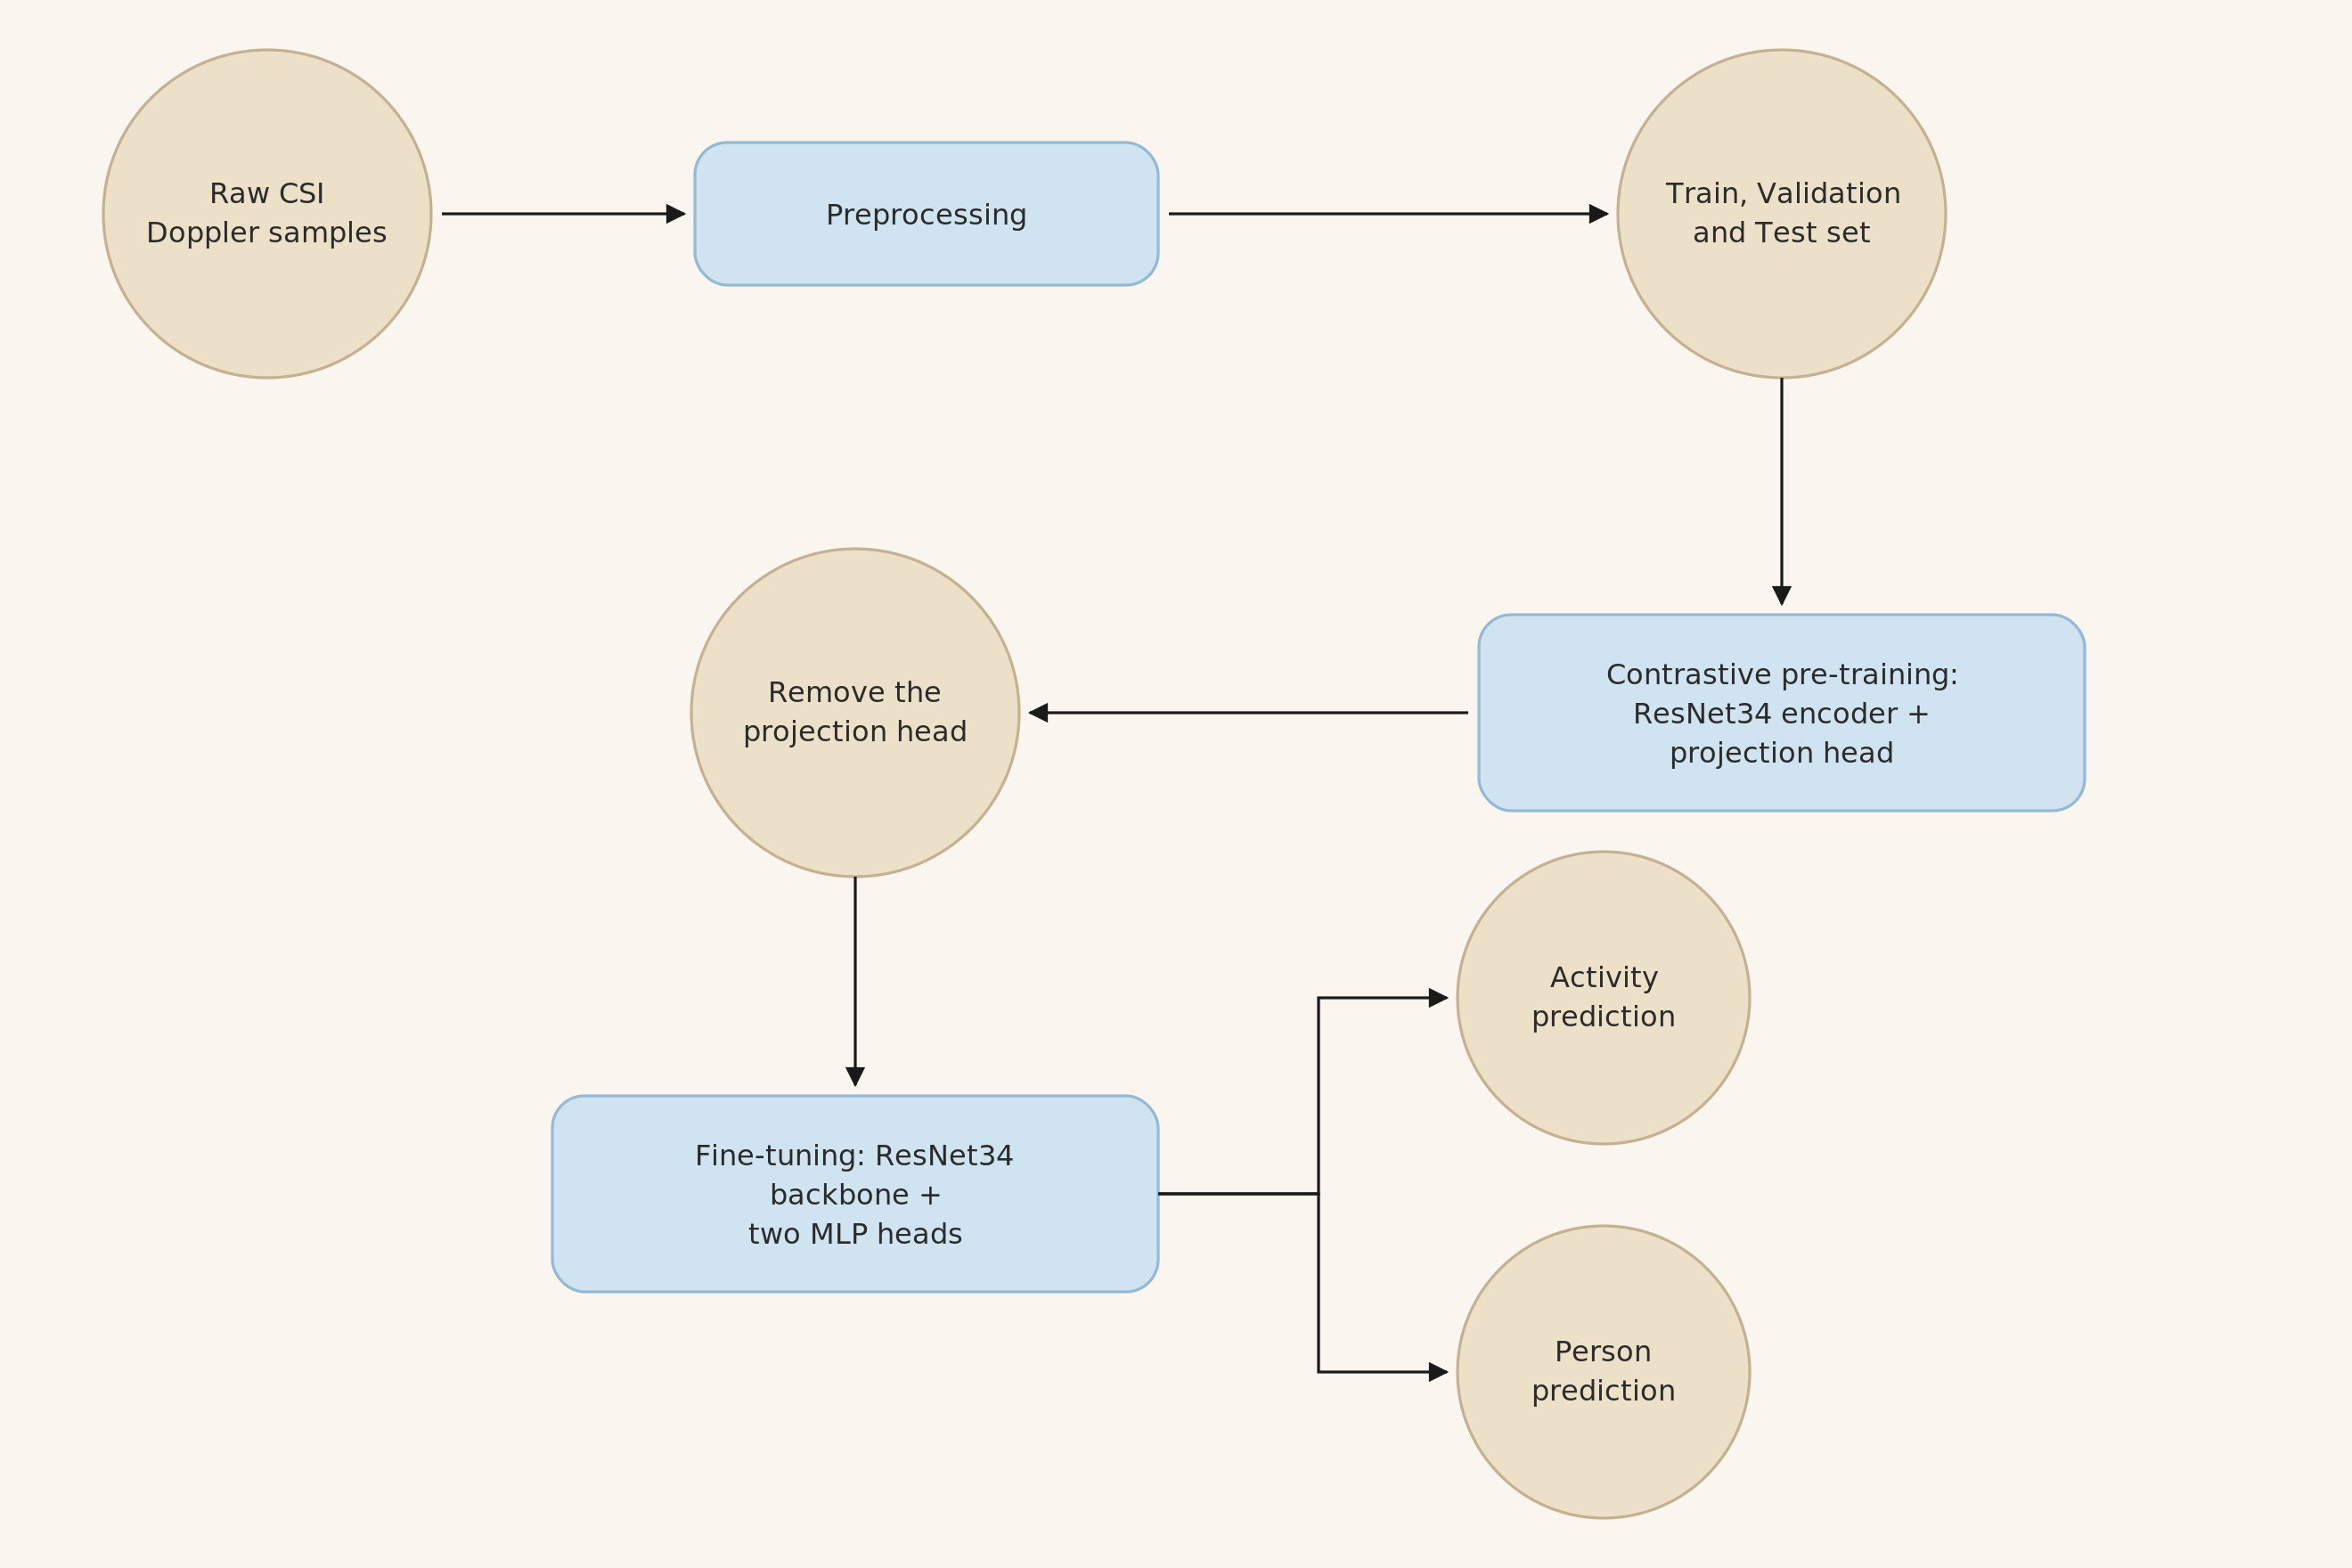
\includegraphics[width=0.3\textwidth]{images/pipeline_diagram.png}
    \caption{Pipeline of the self-supervised contrastive approach}
    \label{fig:FirstPipeline}
\end{figure}
\begin{figure}[h]
    \centering
    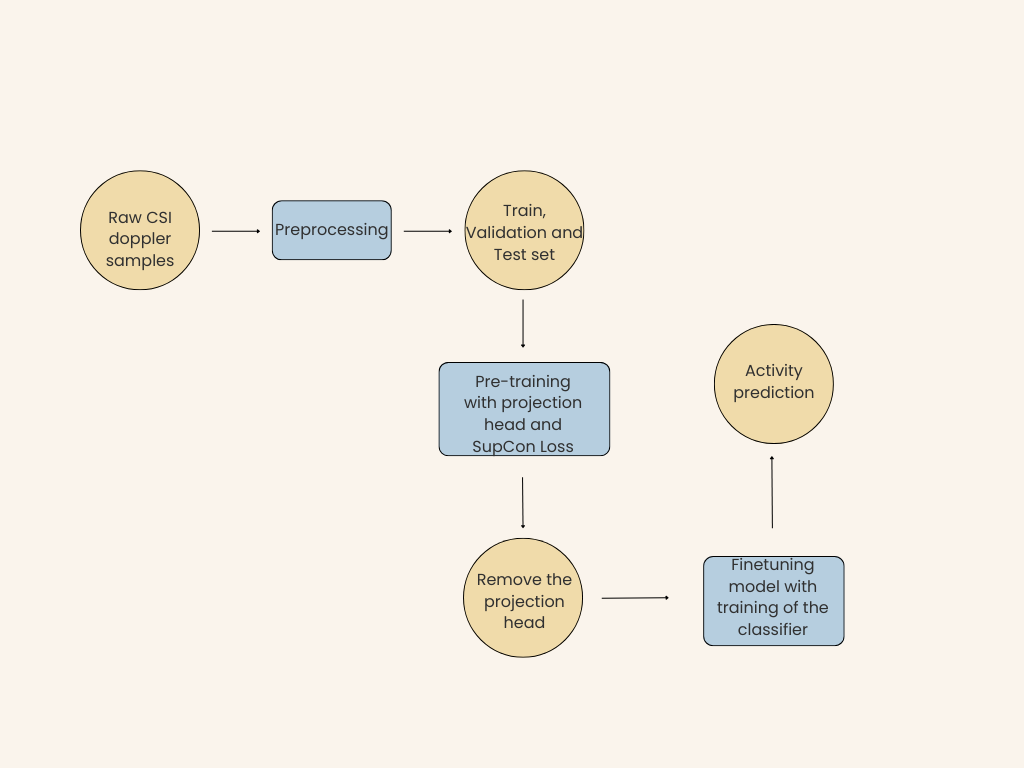
\includegraphics[width=0.3\textwidth]{images/White Beige Minimal Flowchart Diagram Graph.png}
    \caption{Pipeline of the supervised contrastive approach}
    \label{fig:SupCon}
\end{figure}

\section{Signals and Features}


In this work, we employ a preprocessed dataset of Doppler traces \cite{dataset, data}. The original data collection relies on two strategically positioned monitoring devices to capture reliable Doppler shift estimates. Specifically, the underlying Wi-Fi infrastructure utilizes Orthogonal Frequency Division Multiplexing (OFDM) to transmit data across $K$ partially overlapping, orthogonal sub-channels. At the receiver, amplitude and phase are estimated for each sub-channel and stored in a Channel State Information (CSI) matrix. This complex matrix characterizes the Channel Frequency Response (CFR) along every receiving antenna. Subsequently, a sanitization step is executed to filter hardware-induced phase offsets. This procedure is strictly necessary, as these inherent anomalies affecting standard Wi-Fi transmissions would otherwise overwhelm and obscure the subtle variations required for the analysis. 


\\

Each Doppler vector is obtained by applying a Fourier transform to a short block of
consecutive channel estimates, and describes how the reflected power is distributed
over the velocities of the scatterers in the scene. The transform is evaluated on 100
points, which sets the number of velocity bins covering the unambiguous velocity range
of about +/- 5 m/s. A new Doppler vector is computed for every received packet, and 340
consecutive vectors, corresponding to roughly two seconds of channel observation, are
stacked along the time axis. Each sample provided to the network is therefore a 100x340
Doppler spectrogram, in which the vertical axis represents velocity and the horizontal
axis represents time \cite{sharp}. The spectrograms of the various possible activities included in the dataset are shown in Fig.~\ref{fig:Spectrograms}.

\begin{figure}[h]
    \centering
    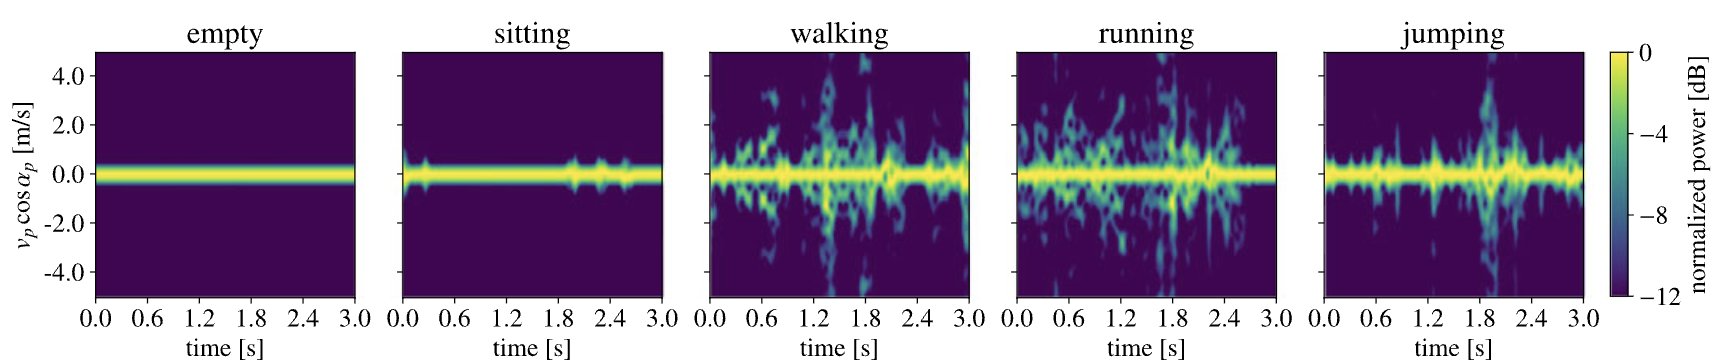
\includegraphics[width=0.5\textwidth]{images/spectrograms.png}
    \caption{Doppler spectrograms for different cases \cite{sharp}}
    \label{fig:Spectrograms}
\end{figure}

\\

The dataset is structured into seven distinct sets, each containing various combinations of subjects, environments, and activities. In the first approach, the data from these sets were partitioned into 60\% for training, 20\% for validation, and 20\% for testing, with the exception of Set 6. This latter set was strictly reserved as a hold-out set, remaining completely unseen by the network. During the self-supervised training phase, a data augmentation pipeline is applied independently to the Doppler spectrogram of each antenna. Specifically, following an initial per-sample standardization (yielding zero mean and unit variance), the signals are subjected to a stochastic sequence of transformations. These operations include circular time shifting, temporal and frequency masking on the Doppler axis, random amplitude scaling, additive Gaussian noise injection, and random patch erasing. 

In the second approach, we used only the first set as training set (still dividing it in 60\% training, 20\% validation and 20\% testing) while the sets from 2 to 7 are used for the testing. Furthermore, in this second approach no transformation is applied to the Doppler spectrogram.

\section{Learning Framework}

The first framework employs a two-stage training strategy for the network. Initially, a self-supervised pre-training phase is conducted to enable the network to learn optimal embeddings for the input signals. Subsequently, a fine-tuning phase is performed on two dedicated heads: one for Person Identification (PI) and another for Activity Recognition (AR).
\subsection{Self-Supervised Contrastive approach architecture}
As the network backbone, both an Inception architecture, similar to the one employed in SHARP \cite{sharp}, and a ResNet-34 \cite{ResNet-34} were evaluated. The former, however, yielded sub-optimal results and was subsequently discarded, likely due to its insufficient network depth. Conversely, the ResNet-34 architecture demonstrated superior performance, as its deeper structure and residual connections facilitated the extraction of more complex hierarchical features from the spectrograms while mitigating the vanishing gradient problem.
\subsection{Phase 1: self-supervised contrastive pre-training}
No label is used in this stage: each window is a distinct instance and its
four antennas act as \emph{natural views} of the same event, each augmented
independently with the pipeline described above. A temporary projection head
maps the backbone features into a $128$-dimensional $L_2$-normalized space,
where the inner product coincides with the cosine similarity, and is
discarded once pre-training is complete.

The starting point is the NT-Xent loss of SimCLR \cite{SimCLR}, which assumes two
views per instance and therefore a single positive per anchor. Since each
window here produces $V=4$ views, we adopt a \emph{multi-positive}
formulation: for a batch of $N$ windows we obtain $M=N\cdot V$ embeddings and,
for the anchor $i$, the positive set $P(i)$ collects the remaining $V-1$ views
of the same window, while every other row of the batch acts as a negative.
Denoting by $\mathbf{z}_i$ the normalized projection of view $i$ and by $\tau$
the temperature, the loss is

\begin{equation}
\mathcal{L} = \frac{1}{M}\sum_{i=1}^{M}
\frac{-1}{|P(i)|}\sum_{p\in P(i)}
\log\frac{\exp\!\left(\mathbf{z}_i^{\top}\mathbf{z}_p/\tau\right)}
{\displaystyle\sum_{a\neq i}\exp\!\left(\mathbf{z}_i^{\top}\mathbf{z}_a/\tau\right)},
\label{eq:ntxent_multiview}
\end{equation}

where the denominator runs over the whole batch except the anchor itself,
whose self-similarity is masked out before the
$\log\text{-}\mathrm{softmax}$ normalization.

This is the same multi-positive form as the Supervised Contrastive loss, but
the grouping is given by the \emph{window identity} instead of the class
label, so the supervision stays entirely self-generated. Averaging the
log-ratio \emph{outside} the logarithm makes the gradient of each positive
independent of $|P(i)|$, and the four antennas are exploited jointly rather
than in pairs, giving three positives and $M-V$ negatives per anchor in a
single forward pass. Optimization uses AdamW ($\eta=2\cdot10^{-4}$, weight
decay $10^{-4}$) with cosine annealing down to $\eta/50$, batches of $64$
windows ($256$ views) and $\tau=0.15$, for $100$ epochs.
\subsection{Phase 2: two-head fine-tuning}

The projection head is discarded and the pre-trained backbone is reused as a
shared feature extractor for two parallel MLP heads,
one for Activity Recognition (5 classes) and one for Person Identification.
Both are supervised with a categorical cross-entropy and optimized jointly as

\begin{equation}
\mathcal{L}_{\mathrm{FT}} =
\mathcal{L}_{\mathrm{CE}}\!\left(\hat{y}_{\mathrm{AR}}, y_{\mathrm{AR}}\right)
+ \lambda\,
\mathcal{L}_{\mathrm{CE}}\!\left(\hat{y}_{\mathrm{PI}}, y_{\mathrm{PI}}\right),
\qquad \lambda = 1,
\label{eq:twohead_loss}
\end{equation}

so that the shared representation is forced to retain both the activity
dynamics and the subject-specific gait signature; the weight $\lambda$
balances the two tasks and is kept at $1$, since neither objective is
treated as auxiliary.

Fine-tuning proceeds in two steps. First a \emph{linear probe}: the backbone
is frozen (its batch-normalization statistics included) and only the two heads
are trained for $15$ epochs with AdamW ($\eta=10^{-3}$, weight decay
$10^{-3}$), which measures how linearly separable the self-supervised features
already are and prevents the randomly initialized heads from corrupting them.
Then a \emph{full fine-tune}: the backbone is unfrozen and the whole network is
trained for at most $10$ epochs with a ten times smaller learning rate
($\eta=10^{-4}$, weight decay $10^{-4}$). Model selection uses the sum of the
validation accuracies of the two heads, with early stopping after $5$ epochs
without improvement and restoration of the best checkpoint.\\\\
\setcounter{subsection}{0}
\subsection{Supervised Contrastive approach architecture}
The framework of the second approach adopts a two-stage transfer learning paradigm: a supervised contrastive learning, followed by a specific fine-tuning phase for the classification task.
The core of this approach is still the architecture used in SHARP \cite{sharp} with the primary building block being \textit{ReductionABlockSmall}, which utilizes pooling branches and parallel convolution in order to extract multi scale features while reducing the spacial and temporal dimensions of the input.
\subsubsection{Phase 1: supervised contrastive pre-training}
To extract robust representations, we employ the Supervised-Contrastive Loss (SupCon Loss)
\begin{equation}
\mathcal{L}_{\text{out}}^{\text{sup}}
=
\sum_{i\in I}
\frac{-1}{|P(i)|}
\sum_{p\in P(i)}
\log
\frac{
\exp\left(\boldsymbol{z}_i \cdot \boldsymbol{z}_p / \tau\right)
}{
\sum\limits_{a\in A(i)}
\exp\left(\boldsymbol{z}_i \cdot \boldsymbol{z}_a / \tau\right)
}.
\end{equation}
the goal is to pull embeddings of the same activity class closer together in the latent space while pushing apart embeddings from different classes. Then a temporary \textit{Projection Head} is attached to the backbone to map high-dimensional features into a 128-dimensional L2-normalized space, where the loss is calculated. The optimization consists in a 20 epochs training using the Adam optimizer with a learning rate of $10^{-4}$ and a temperature parameter $\tau=0.07$.
\subsubsection{Phase 2: Fine-Tuning for classification}
Once pre-training is complete the \textit{Projection Head} is removed and replaced by a \textit{linear classification Head}, furthermore the weights of the backbone are freezed and only the final fully connected layer is trained. In this phase a \textit{Categorical Cross Entropy Loss} is used to guide the training and map the extracted features into the 5 target activity classes. In the end, to prevent overfitting, a Dropout layer (0.2 rate) is used before the final one and training is governed by an \textit{Early-Stopping} mechanism based on the validation accuracy.
\subsubsection{Decision Fusion}
Since the setup utilizes 4 different antennas to obtain the signals, the framework implements a \textit{Decision Fusion} strategy where, instead of relying on a single antenna prediction, the model aggregates the output of all the antennas associated with the same time slot. The final class assignment is determined using a \textit{Majority Voting} criteria or, in case of tie, by evaluating the sum of the predicted logits across all antennas to ensure the maximum reliability.
\label{sec:processing_architecture}